\begin{savequote}[45mm]
\ascii{Any fool can write code that a computer can understand. Good programmers write code that humans can understand.}
\qauthor{\ascii{- Martin Flower}}
\end{savequote}

\chapter{变量} 
\label{ch:variable}

\begin{content}

\ascii{Variable}是一个特殊的\ascii{OP},它拥有状态\ascii{(Stateful)}。从实现技术探究,\ascii{Variable}的\ascii{Kernel}实现直接持有一个\ascii{Tensor}实例,其生命周期与变量一致。相对于普通的\ascii{Tensor}实例,其生命周期仅对本次迭代\ascii{(Step)}有效;而\ascii{Variable}对多个迭代都有效,甚至可以存储到文件系统,或从文件系统中恢复。

\end{content}

\section{实战:线性模型}

\begin{content}

以一个简单的线性模型为例(为了简化问题,此处省略了训练子图)。首先,使用\code{tf.placeholder}定义模型的输入,然后定义了两个全局变量,同时它们都是训练参数,最后定义了一个简单的线性模型。

\begin{leftbar}
\begin{python}
x  = tf.placeholder(tf.float32, [None, 784])
W = tf.Variable(tf.zeros([784,10]), name='W')
b = tf.Variable(tf.zeros([10]), name='b') 
y = tf.matmul(x, W) + b
\end{python}
\end{leftbar}

在使用变量之前,必须对变量进行初始化。按照习惯用法,使用\code{tf.global\_variables}
\code{\_initializer()}将所有全局变量的初始化器汇总,并对其进行初始化。

\begin{leftbar}
\begin{python}
init = tf.global_variables_initializer()

with tf.Session() as sess:
  sess.run(init)
\end{python}
\end{leftbar}

按照既有经验,其计算图大致如\refig{tf-linear-model}所示。

\begin{figure}[!h]
\centering
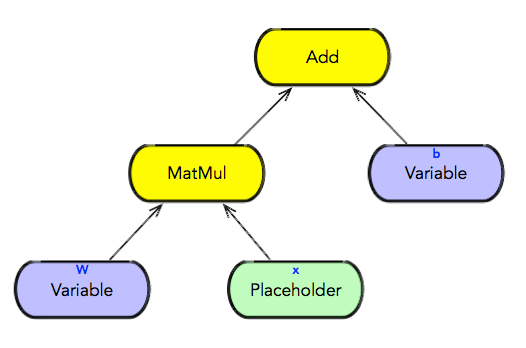
\includegraphics[width=0.6\textwidth]{figures/tf-linear-model.png}
\caption{计算图: 线性加权和}
 \label{fig:tf-linear-model}
\end{figure}

事实上,正如\refig{tf-real-linear-model}所示,实际的计算图要复杂得多,让我们从头说起。

\begin{figure}[!h]
\centering
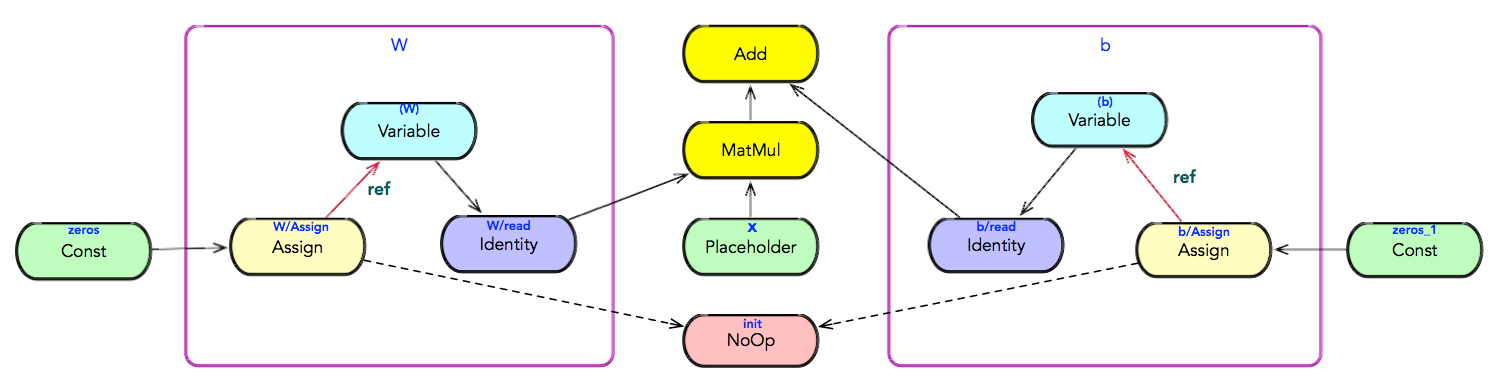
\includegraphics[width=1.0\textwidth]{figures/tf-real-linear-model.png}
\caption{计算图: 线性加权和}
 \label{fig:tf-real-linear-model}
\end{figure}

\end{content}

\section{初始化模型}

\begin{content}

\ascii{Variable}是一个特殊的OP,它拥有状态\ascii{(Stateful)}。如果从实现技术探究,\ascii{Variable}的K\ascii{ernel}实现直接持有一个\ascii{Tensor}实例,其生命周期与\ascii{Variable}一致。相对于普通的\ascii{Tensor}实例,其生命周期仅对本次迭代\ascii{(Step)}有效;而\ascii{Variable}对多个迭代\ascii{(Step)}都有效,甚至可以持久化到文件系统,或从文件系统中恢复。

\subsection{操作变量}

存在几个操作\ascii{Variable}的特殊OP用于修改变量的值,例如\ascii{Assign, AssignAdd}等。\ascii{Variable}所持有的\ascii{Tensor}以引用的方式输入到\ascii{Assign}中,\ascii{Assign}根据初始值\ascii{(Initial Value)}或新值,就地修改\ascii{Tensor}内部的值,最后以引用的方式输出该\ascii{Tensor}。

从设计角度看,\ascii{Variable}可以看做\ascii{Tensor}的包装器,\ascii{Tensor}所支持的所有操作都被\ascii{Variable}重载实现。也就是说,\ascii{Variable}可以出现在\ascii{Tensor}的所有地方。例如,

\begin{leftbar}
\begin{python}
# Create a variable
W = tf.Variable(tf.zeros([784,10]), name='W')

# Use the variable in the graph like any Tensor.
y = tf.matmul(x, W)

# The overloaded operators are available too.
z = tf.sigmoid(w + y)

# Assign a new value to the variable with assign/assign\_add.
w.assign(w + 1.0)
w.assign_add(1.0)
\end{python}
\end{leftbar}

\subsection{初始值}

一般地,在使用变量之前,必须对变量进行初始化。事实上,\ascii{TensorFlow}设计了一个精巧的变量初始化模型。\ascii{Variable}根据初始值\ascii{(Initial Value)}推演\ascii{Variable}的数据类型,并确定\ascii{Tensor}的形状\ascii{(Shape)}。

例如,\code{tf.zeros}称为\ascii{Variable}的初始值,它确定了\ascii{Variable}的类型为\code{int32},且\ascii{Shape}为\code{[784, 10]}。

\begin{leftbar}
\begin{python}
# Create a variable.
W = tf.Variable(tf.zeros([784,10]), name='W')
\end{python}
\end{leftbar}

如下表所示,构造变量初始值的常见\ascii{OP}包括:

\subsection{初始化器}

另外,变量通过初始化器\ascii{(Initializer)}在初始化期间,将初始化值赋予\ascii{Variable}内部所持有\ascii{Tensor},完成\ascii{Variable}的就地修改。

在变量使用之前,必须保证变量被初始化器已初始化。事实上,变量初始化过程,即运行变量的初始化器。

证如上例\code{W}的定义,可以如下完成\code{W}的初始化。此处,\code{W.initializer}实际上为\ascii{Assign}的\ascii{OP},这是\ascii{Variable}默认的初始化器。

\begin{leftbar}
\begin{python}
# Run the variable initializer.
with tf.Session() as sess:
  sess.run(W.initializer)
\end{python}
\end{leftbar}

一旦完成\ascii{Variable}的初始化,其类型与值得以确定。随后可以使用\ascii{Assign}族的\ascii{OP}(例如\ascii{Assign, AssignAdd}等)修改\ascii{Variable}的值。

需要注意的是,在\ascii{TensorBoard}中展示\ascii{Assign}的输入,其边使用特殊的\ascii{ref}标识。数据流向与之刚好相反,否则计算图必然出现环,显然违反了\ascii{DAG}(有向无环图)的基本需求。

\subsection{快照}

如果要读取变量的值,则通过\ascii{Identity}恒等变化,直接输出变量所持有的\ascii{Tensor}。\ascii{Identity}去除了\ascii{Variable}的引用标识,同时也避免了内存拷贝。

\ascii{Identity}操作\ascii{Variable}常称为一个快照\ascii{(Snapshot)},表示\ascii{Variable}当前的值。

事实上,通过\ascii{Identity}将\ascii{Variable}转变为普通的\ascii{Tensor},使得它能够兼容所有\ascii{Tensor}的操作。


\subsection{变量子图}

例如,变量\ascii{W}的定义如下。

\begin{leftbar}
\begin{python}
W = tf.Variable(tf.zeros([784,10]), name='W')
\end{python}
\end{leftbar}

\code{tf.zeros([784,10])}常称为初始值,它通过初始化器\ascii{Assign},将\code{W}内部持有的\ascii{Tensor}以引用的形式就地修改为该初始值;同时,\ascii{Identity}去除了\ascii{Variable}的引用标识,实现了\ascii{Variable}的读取。

\begin{figure}[!h]
\centering
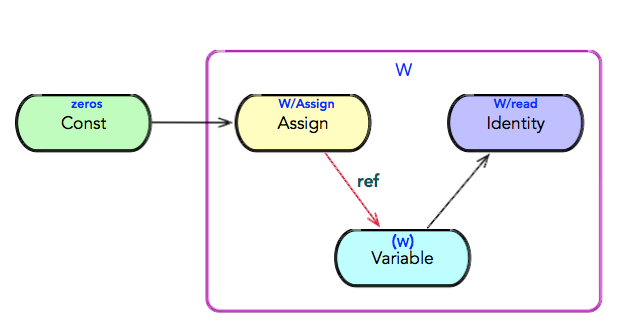
\includegraphics[width=0.8\textwidth]{figures/variable-initialization-model.png}
\caption{变量子图}
 \label{fig:variable-initialization-model}
\end{figure}


\subsection{初始化过程}

更为常见的是,通过调用\code{tf.global\_variables\_initializer()}将所有变量的初始化器进行汇总,然后启动\ascii{Session}运行该\ascii{OP}。

\begin{leftbar}
\begin{python}
init = tf.global_variables_initializer()
\end{python}
\end{leftbar}

事实上,搜集所有全局变量的初始化器的\ascii{OP}是一个\ascii{NoOp},即不存在输入,也不存在输出。所有变量的初始化器通过控制依赖边与该\ascii{NoOp}相连,保证所有的全局变量被初始化。

\begin{figure}[!h]
\centering
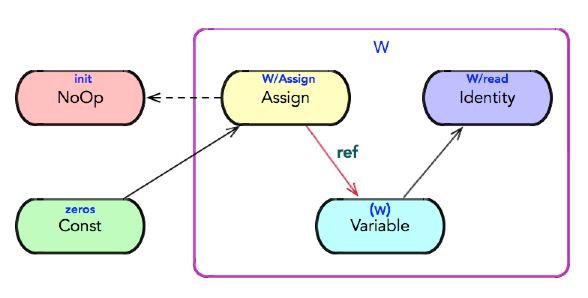
\includegraphics[width=0.8\textwidth]{figures/variable-initialization-no-op.png}
\caption{初始化OP}
 \label{fig:variable-initialization-no-op}
\end{figure}

\subsection{同位关系}

同位关系是一种特殊的设备约束关系。显而易见,\ascii{Assign, Identity}这两个\ascii{OP}与\ascii{Variable}关系极其紧密,分别实现了变量的修改与读取。因此,它们必须与\ascii{Variable}在同一个设备上执行;这样的关系,常称为同位关系\ascii{(Colocation)}。

可以在\ascii{Assign/Identity}节点上指定\code{\_class}属性值:\code{[s: "loc:@W"]},它表示这两个\ascii{OP}与\code{W}放在同一个设备上运行。

例如,以\code{W/read}节点为例,该节点增加了\code{\_class}属性,指示与\code{W}的同位关系。

\begin{leftbar}
\begin{python}
node {
  name: "W/read"
  op: "Identity"
  input: "W"
  attr {
    key: "T"
    value {
      type: DT_FLOAT
    }
  }
  attr {
    key: "_class"
    value {
      list {
        s: "loc:@W"
      }
    }
  }
}
\end{python}
\end{leftbar}

\subsection{初始化依赖}

如果一个变量初始化需要依赖于另外一个变量的初始值,则需要特殊地处理。例如,变量\code{V}的初始值依赖于\code{W}的初始值,可以通过\code{W.initialized\_value()}指定。

\begin{leftbar}
\begin{python}
W = tf.Variable(tf.zeros([784,10]), name='W')
V = tf.Variable(W.initialized_value(), name='V')
\end{python}
\end{leftbar}

事实上,两者通过\ascii{Identity}衔接,并显式地添加了依赖控制边,保证\code{W}在\code{V}之前初始化。此处,存在两个\ascii{Identity}的\ascii{OP},但职责不一样,它们分别完成初始化依赖和变量读取。


\begin{figure}[!h]
\centering
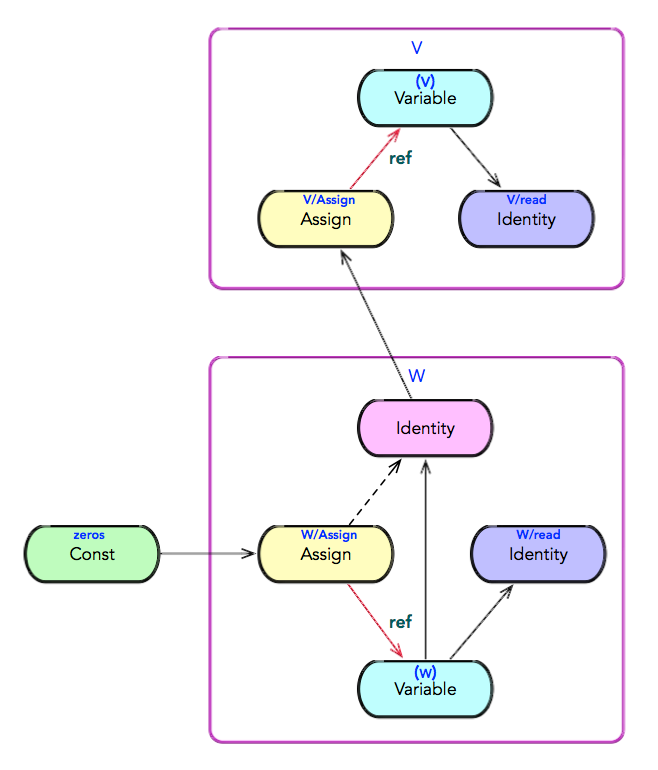
\includegraphics[width=0.8\textwidth]{figures/variable-initialization-dependency-1.png}
\caption{初始化依赖}
 \label{fig:variable-initialization-dependency-1}
\end{figure}

同样地,可以通过调用\code{tf.global\_variables\_initializer()}将变量的所有初始化器进行汇总,然后启动\ascii{Session}完成所有变量的初始化。

\begin{leftbar}
\begin{python}
init = tf.global_variables_initializer()
\end{python}
\end{leftbar}

按照依赖关系,因为增加了\code{W/Assign}与\code{Identity}之间的控制依赖边,从而巧妙地实现了\code{W}在\code{V}之前完成初始化,并通过\code{W}当前的初始化值,最终完成\code{V}的初始化。

\begin{figure}[!h]
\centering
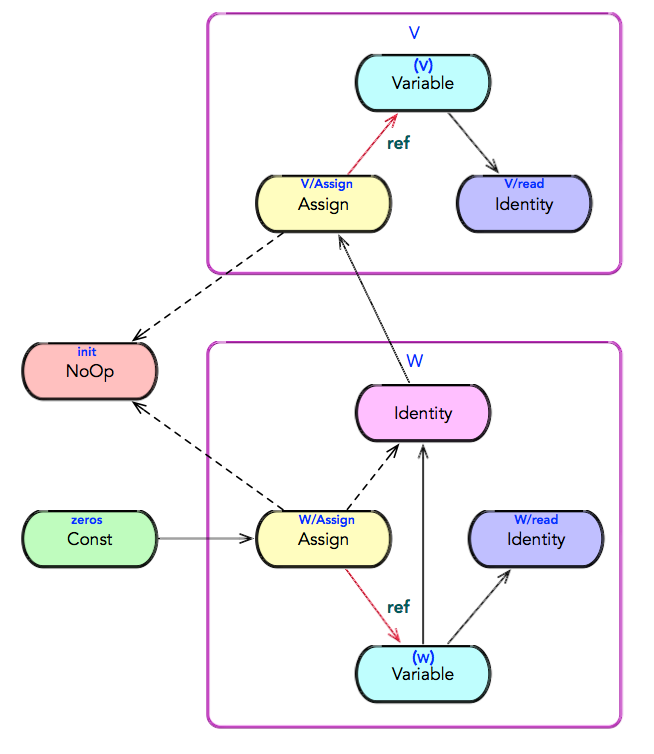
\includegraphics[width=0.8\textwidth]{figures/variable-initialization-dependency-2.png}
\caption{初始化OP}
 \label{fig:variable-initialization-dependency-2}
\end{figure}

\subsection{初始化器列表}

可以使用\code{variables\_initializer}构建变量列表的初始化器列表。其中,\code{group}将构造一个仅控制依赖于\code{\_initialier\_list()}的\ascii{NoOP}。

\begin{leftbar}
\begin{python}
def variables_initializer(var_list, name="init"):
  def _initialier_list():
    return *[v.initializer for v in var_list]
  return control_flow_ops.group(_initialier_list(), name=name)
\end{python}
\end{leftbar}

例如,全局变量列表的初始化器列表可以如下构造。

\begin{leftbar}
\begin{python}
def global_variables_initializer():
  return variables_initializer(global_variables())
\end{python}
\end{leftbar}

\end{content}

\section{变量分组}

\begin{content}

默认地,\ascii{Variable}被划分在全局变量和训练变量的集合中。正如上例,\code{W, V}自动划分至全局变量和训练变量的集合中。

\subsection{全局变量}

可以通过\code{tf.global\_variables()}方便地检索全局变量的集合。在分布式环境中,全局变量能在不同的进程间实现参数共享。

\begin{leftbar}
\begin{python}
def global_variables():
  return ops.get_collection(ops.GraphKeys.GLOBAL_VARIABLES)
\end{python}
\end{leftbar}

\subsection{本地变量}

可以通过\code{tf.local\_variables()}方便地检索本地变量的集合。

\begin{leftbar}
\begin{python}
def local_variables():
  return ops.get_collection(ops.GraphKeys.LOCAL_VARIABLES)
\end{python}
\end{leftbar}

可以使用\code{local\_variable}的语法糖,构建一个本地变量。

\begin{leftbar}
\begin{python}
def local_variable(initial_value, validate_shape=True, name=None):
  return variables.Variable(
      initial_value, trainable=False,
      collections=[ops.GraphKeys.LOCAL_VARIABLES],
      validate_shape=validate_shape, name=name)
\end{python}
\end{leftbar}

本地变量表示进程内的共享变量,它通常不需要做断点恢复\ascii{(Checkpoint)},仅用于临时的计数器的用途。例如,在分布式环境中,使用本地变量记录该进程已读数据的\ascii{Epoch}数目。

\subsection{训练变量}

可以通过\code{tf.trainable\_variables()}检索训练变量的集合。在机器学习中,训练变量表示模型参数。

\begin{leftbar}
\begin{python}
def trainable_variables():
  return ops.get_collection(ops.GraphKeys.TRAINABLE_VARIABLES)
\end{python}
\end{leftbar}

\subsection{global\_step}

\code{global\_step}是一个特殊的\ascii{Variable},它不是训练变量,但它是一个全局变量。在分布式环境中,\code{global\_step}常用于追踪已运行\ascii{step}的次数,并在不同进程间实现数据的同步。

创建一个\code{global\_step}可以使用如下函数:

\begin{leftbar}
\begin{python}
def create_global_step(graph=None):
  graph = ops.get_default_graph() if graph is None else graph
  with graph.as_default() as g, g.name_scope(None):
    collections = [GLOBAL_VARIABLES, GLOBAL_STEP]
    return variable(
        GLOBAL_STEP,
        shape=[],
        dtype=dtypes.int64,
        initializer=init_ops.zeros_initializer(),
        trainable=False,
        collections=collections)
\end{python}
\end{leftbar}

\end{content}

\section{源码分析:构造变量}

\begin{content}

为了简化代码实现,此处对\ascii{Variable}做了简单的重构。

\begin{leftbar}
\begin{python}
class Variable(object):
  def __init__(self, initial_value=None, trainable=True,
    collections=None, name=None, dtype=None):
    with ops.name_scope(name, "Variable", [initial_value]) as name:
      self._cons_initial_value(initial_value, dtype)
      self._cons_variable(name)
      self._cons_initializer()
      self._cons_snapshot()
    self._cons_collections(trainable, collections)
\end{python}
\end{leftbar}

构造\ascii{Variable}实例,基本包括如下几个步骤:

\subsection{构造初始值}

\begin{leftbar}
\begin{python}
  def _cons_initial_value(self, initial_value, dtype):
    self._initial_value = ops.convert_to_tensor(
        initial_value, name="initial_value", dtype=dtype)
\end{python}
\end{leftbar}

\subsection{构造变量OP}

\ascii{Variable}根据初始值的类型和大小完成自动推演。

\begin{leftbar}
\begin{python}
  def _cons_variable(self, name):
    self._variable = state_ops.variable_op_v2(
      self._initial_value.get_shape(),
      self._initial_value.dtype.base_dtype,
      name=name)
\end{python}
\end{leftbar}

\subsection{构造初始化器}

\ascii{Variable}的初始化器本质上是一个\ascii{Assign},它持有\ascii{Variable}的引用,并使用初始值就地修改变量本身。

\begin{leftbar}
\begin{python}
  def _cons_initializer(self):
    self._initializer_op = state_ops.assign(
      self._variable,
      self._initial_value).op
\end{python}
\end{leftbar}

\subsection{构造快照}

\ascii{Variable}的快照本质上是一个\ascii{Identity},表示\ascii{Variable}的当前值。

\begin{leftbar}
\begin{python}
  def _cons_snapshot(self):
    with ops.colocate_with(self._variable.op):
      self._snapshot = array_ops.identity(
        self._variable, name="read")
\end{python}
\end{leftbar}

\subsection{变量分组}

默认地,\ascii{Variable}被划分在全局变量的集合中;如果\code{trainable}为真,则表示该变量为训练参数,并将其划分到训练变量的集合中。

\begin{leftbar}
\begin{python}
  def _cons_collections(self, trainable, collections)
    if collections is None:
      collections = [GLOBAL_VARIABLES]
    if trainable and TRAINABLE_VARIABLES not in collections:
      collections = list(collections) + [TRAINABLE_VARIABLES]
    ops.add_to_collections(collections, self)
\end{python}
\end{leftbar}

\end{content}